\documentclass[12pt,a4paper]{article}
\usepackage{amsmath,amsthm,amssymb,mathtools}
\usepackage{tikz}
\usetikzlibrary{arrows.meta,positioning,shapes.geometric,calc,fit,backgrounds}
\usepackage{graphicx}
\usepackage{booktabs,tabularx,multirow}
\usepackage[ruled,vlined,linesnumbered]{algorithm2e}
\usepackage[most]{tcolorbox}
\usepackage{hyperref}
\usepackage[capitalize,noabbrev]{cleveref}
\usepackage[margin=1in]{geometry}
\usepackage{fancyhdr}
\usepackage{enumitem}
\usepackage{xcolor}

%% ── tcolorbox environments ──────────────────────────────────────────────────
\newtcolorbox{keyinsight}[1][]{colback=blue!5!white,colframe=blue!75!black,
  fonttitle=\bfseries,title=Key Insight,#1}
\newtcolorbox{example}[1][]{colback=green!5!white,colframe=green!75!black,
  fonttitle=\bfseries,title=Example,#1}
\newtcolorbox{warningbox}[1][]{colback=red!5!white,colframe=red!75!black,
  fonttitle=\bfseries,title=Warning,#1}

%% ── amsthm environments ─────────────────────────────────────────────────────
\newtheorem{theorem}{Theorem}[section]
\newtheorem{lemma}[theorem]{Lemma}
\newtheorem{definition}{Definition}[section]
\newtheorem{remark}{Remark}[section]

%% ── page style ───────────────────────────────────────────────────────────────
\pagestyle{fancy}
\fancyhf{}
\rhead{Deep Learning -- Session 07}
\lhead{Backpropagation \& Gradient Descent}
\cfoot{\thepage}

\hypersetup{
  colorlinks=true,
  linkcolor=blue!70!black,
  urlcolor=blue!70!black
}

%% ── convenience macros ───────────────────────────────────────────────────────
\newcommand{\Loss}{\mathcal{L}}
\newcommand{\ReLU}{\operatorname{ReLU}}
\newcommand{\yhat}{\hat{y}}
\newcommand{\pderiv}[2]{\dfrac{\partial #1}{\partial #2}}

% ─────────────────────────────────────────────────────────────────────────────
\begin{document}

%% ── Title page ───────────────────────────────────────────────────────────────
\begin{titlepage}
  \centering
  \vspace*{2cm}
  {\LARGE\bfseries Deep Learning: Advanced ANN Concepts\par}
  \vspace{0.5cm}
  {\large Lecture Notes -- Session 07\par}
  \vspace{1.5cm}
  \rule{\linewidth}{0.5pt}\\[0.4cm]
  {\huge\bfseries Backpropagation Worked Example\\[0.3cm]
   \& Gradient Descent\par}
  \rule{\linewidth}{0.5pt}\\[1.5cm]

  \begin{tabular}{ll}
    \textbf{Session}     & 07 \\[4pt]
    \textbf{Topic}       & Backpropagation numerical example; chain-rule derivation \\
                         & for all 9 parameters; learning rate; gradient descent \\[4pt]
    \textbf{Deck}        & \texttt{03-DL-ANNAdvancedConcepts} \\[4pt]
    \textbf{Instructors} & Prof.\ S R M Prasanna \& Dr.\ Sunil Saumya \\[4pt]
    \textbf{Institute}   & IIIT Dharwad \\[4pt]
    \textbf{Duration}    & $\approx 1$h $39$m \\[4pt]
    \textbf{Video}       & \url{https://vimeo.com/1144571367} \\
  \end{tabular}

  \vfill
  {\large\itshape Course: Deep Learning -- Advanced ANN Concepts\par}
\end{titlepage}

%% ── Table of Contents ────────────────────────────────────────────────────────
\tableofcontents
\newpage

% =============================================================================
\section{Introduction}
\label{sec:intro}
% =============================================================================

Session~07 sits at the boundary between \emph{first-level} and
\emph{advanced-level} understanding of artificial neural networks.
The first six sessions established the perceptron, multi-layer perceptrons,
forward propagation, and the conceptual role of backpropagation.
This session consolidates that foundation by working through every arithmetic
step of a complete backpropagation pass, then transitions to the key concepts
needed to train networks reliably in practice:

\begin{itemize}[leftmargin=2em]
  \item A full numerical forward pass on a 2-input, 2-hidden-neuron,
        1-output network (IQ/CGPA $\to$ placement-salary prediction).
  \item Exact computation of all 9 gradients via the chain rule.
  \item One complete parameter update with learning rate $\eta = 10^{-4}$,
        demonstrating a 92.6\% drop in loss ($54.17 \to 4.006$) in a single
        step.
  \item Intuition behind gradient descent and why the update rule
        $\theta \leftarrow \theta - \eta\,\pderiv{\Loss}{\theta}$ always
        moves toward the minimum.
  \item Three variants of gradient descent --- batch, stochastic, and
        mini-batch --- with trade-off analysis.
  \item PyTorch implementation hints for each variant.
\end{itemize}

The material applies directly to every deeper architecture (CNN, RNN, LSTM)
studied in later sessions: the chain-rule mechanics, the update rule, and the
gradient-descent variants are universal.

% =============================================================================
\section{Background and Prerequisites}
\label{sec:background}
% =============================================================================

\subsection{The Network Architecture}

Throughout this session the instructors use a fixed toy network:
two inputs $x_1, x_2$, two hidden neurons producing activations $h_1, h_2$,
and one linear output neuron $\yhat$.
The task is regression: predict a numeric placement salary (LPA) from
IQ score and CGPA.

\begin{definition}[Feedforward Neural Network -- Session Notation]
\label{def:ffnn}
A \emph{feedforward neural network} with one hidden layer computes:
\begin{align}
  z_k &= \sum_j w_{kj}\,x_j + b_k, \qquad k=1,2 \label{eq:hidden-preact}\\
  h_k &= \ReLU(z_k) = \max(0,\, z_k), \qquad k=1,2 \label{eq:relu}\\
  \yhat &= v_1 h_1 + v_2 h_2 + b_3. \label{eq:output}
\end{align}
The squared-error loss for one sample $(x_1,x_2,y)$ is
\begin{equation}
  \Loss = (\yhat - y)^2. \label{eq:loss}
\end{equation}
\end{definition}

\subsection{Parameter Inventory}

The 9 trainable parameters are:
\[
  \Theta = \{w_{11},\, w_{12},\, w_{21},\, w_{22},\, b_1,\, b_2,\, v_1,\, v_2,\, b_3\}.
\]

\subsection{The ReLU Activation and Its Derivative}

\begin{definition}[ReLU]
\label{def:relu}
$\ReLU(z) = \max(0,z)$, with sub-gradient
\begin{equation}
  \frac{d\,\ReLU}{dz}(z) = \mathbf{1}[z > 0] =
  \begin{cases} 1 & z > 0 \\ 0 & z \leq 0. \end{cases}
  \label{eq:relu-deriv}
\end{equation}
\end{definition}

\begin{keyinsight}
ReLU's derivative is either 0 or 1 --- never a tiny fraction.
This prevents the \emph{vanishing gradient problem} that plagued
sigmoid-based networks, and is the main reason ReLU became the
default hidden-layer activation.
\end{keyinsight}

\subsection{Chain Rule (Univariate)}

For a composed function $\Loss = f(g(\theta))$:
\begin{equation}
  \pderiv{\Loss}{\theta} = \pderiv{\Loss}{g} \cdot \pderiv{g}{\theta}.
  \label{eq:chain-rule}
\end{equation}
Backpropagation applies \cref{eq:chain-rule} recursively, propagating
partial derivatives from the output layer back through each hidden layer.

% =============================================================================
\section{Forward Pass: Numerical Worked Example}
\label{sec:forward}
% =============================================================================

\subsection{Initial Parameter Values}

The session begins with the following hand-crafted initial values
(first row of the toy dataset):

\begin{center}
\begin{tabular}{lll}
\toprule
\textbf{Quantity} & \textbf{Symbol} & \textbf{Value} \\
\midrule
Input 1 (IQ)    & $x_1$ & $80$ \\
Input 2 (CGPA)  & $x_2$ & $8$  \\
Target (LPA)    & $y$   & $3$  \\
\midrule
Hidden weight   & $w_{11}$ & $0.02$ \\
Hidden weight   & $w_{12}$ & $0.50$ \\
Hidden weight   & $w_{21}$ & $0.04$ \\
Hidden weight   & $w_{22}$ & $-0.30$ \\
Hidden bias     & $b_1$    & $1$ \\
Hidden bias     & $b_2$    & $1$ \\
Output weight   & $v_1$    & $1.2$ \\
Output weight   & $v_2$    & $0.8$ \\
Output bias     & $b_3$    & $1$ \\
\bottomrule
\end{tabular}
\end{center}

\subsection{Step-by-Step Computation}

\paragraph{Hidden neuron 1.}
\begin{align}
  z_1 &= w_{11} x_1 + w_{12} x_2 + b_1
       = 0.02\cdot80 + 0.5\cdot8 + 1
       = 1.6 + 4.0 + 1.0 = 6.6, \label{eq:z1}\\
  h_1 &= \ReLU(6.6) = 6.6. \label{eq:h1}
\end{align}

\paragraph{Hidden neuron 2.}
\begin{align}
  z_2 &= w_{21} x_1 + w_{22} x_2 + b_2
       = 0.04\cdot80 + (-0.3)\cdot8 + 1
       = 3.2 - 2.4 + 1.0 = 1.8, \label{eq:z2}\\
  h_2 &= \ReLU(1.8) = 1.8. \label{eq:h2}
\end{align}

\paragraph{Output neuron.}
\begin{align}
  \yhat &= v_1 h_1 + v_2 h_2 + b_3
         = 1.2\cdot6.6 + 0.8\cdot1.8 + 1
         = 7.92 + 1.44 + 1.0 = 10.36. \label{eq:yhat}
\end{align}

\paragraph{Loss.}
\begin{equation}
  \Loss = (\yhat - y)^2 = (10.36 - 3)^2 = (7.36)^2 \approx 54.17.
  \label{eq:loss-val}
\end{equation}

\begin{example}[Why is the initial prediction so poor?]
$x_1 = 80$ is a large number.
With $w_{11} = 0.02$, the pre-activation $z_1 = 6.6$ is already large,
and after multiplying by $v_1 = 1.2$ the network predicts $\yhat = 10.36$
when the target is only $y = 3$.
This illustrates why \emph{input normalisation} is important in practice:
unscaled features cause large pre-activations and correspondingly large
gradients, which destabilise training.
\end{example}

\subsection{Network Diagram}

\cref{fig:network} shows the architecture with the numerical values annotated
on each connection.

\begin{figure}[ht]
\centering
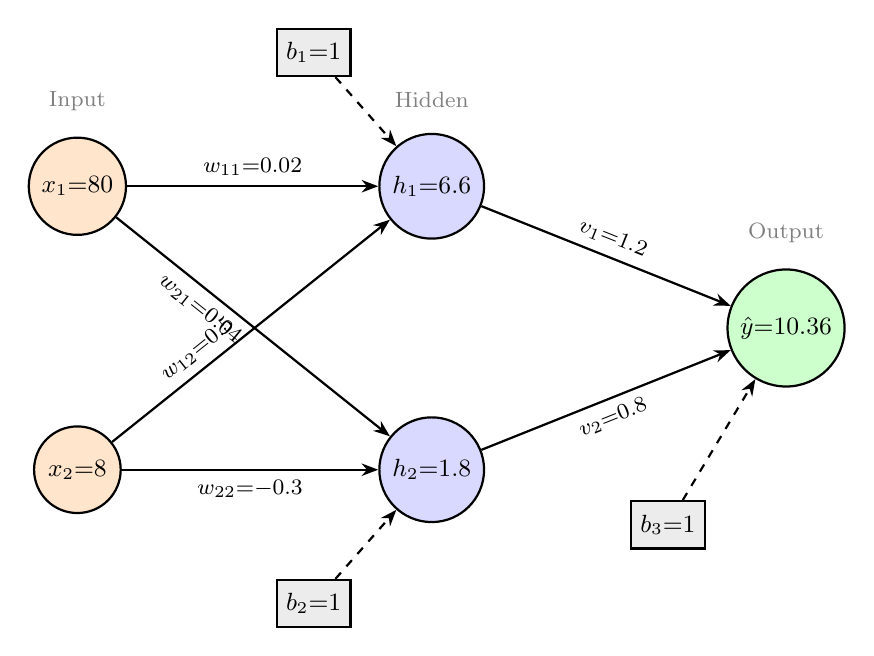
\begin{tikzpicture}[
    neuron/.style={circle,draw,minimum size=1.1cm,thick},
    bias/.style={rectangle,draw,minimum size=0.6cm,fill=gray!15,thick},
    arr/.style={-{Stealth[length=6pt]},thick},
    font=\small
  ]
  %% Input layer
  \node[neuron,fill=orange!20] (x1) at (0, 1.8) {$x_1{=}80$};
  \node[neuron,fill=orange!20] (x2) at (0,-1.8) {$x_2{=}8$};

  %% Hidden layer
  \node[neuron,fill=blue!15]  (h1) at (4.5, 1.8) {$h_1{=}6.6$};
  \node[neuron,fill=blue!15]  (h2) at (4.5,-1.8) {$h_2{=}1.8$};
  \node[bias] (b1) at (3.0, 3.5) {$b_1{=}1$};
  \node[bias] (b2) at (3.0,-3.5) {$b_2{=}1$};

  %% Output layer
  \node[neuron,fill=green!20] (yh) at (9, 0) {$\hat{y}{=}10.36$};
  \node[bias] (b3) at (7.5,-2.5) {$b_3{=}1$};

  %% x1 -> h1, h2
  \draw[arr] (x1) -- node[above,sloped]{\footnotesize$w_{11}{=}0.02$} (h1);
  \draw[arr] (x1) -- node[below,sloped,pos=0.35]{\footnotesize$w_{21}{=}0.04$} (h2);

  %% x2 -> h1, h2
  \draw[arr] (x2) -- node[above,sloped,pos=0.35]{\footnotesize$w_{12}{=}0.5$} (h1);
  \draw[arr] (x2) -- node[below,sloped]{\footnotesize$w_{22}{=}{-}0.3$} (h2);

  %% biases -> hidden
  \draw[arr,dashed] (b1) -- (h1);
  \draw[arr,dashed] (b2) -- (h2);

  %% hidden -> output
  \draw[arr] (h1) -- node[above,sloped]{\footnotesize$v_1{=}1.2$} (yh);
  \draw[arr] (h2) -- node[below,sloped]{\footnotesize$v_2{=}0.8$} (yh);
  \draw[arr,dashed] (b3) -- (yh);

  %% layer labels
  \node[above=0.2cm of x1,gray]  {\footnotesize Input};
  \node[above=0.2cm of h1,gray]  {\footnotesize Hidden};
  \node[above=0.2cm of yh,gray]  {\footnotesize Output};
\end{tikzpicture}
\caption{Two-input, two-hidden-neuron, one-output network with initial
         parameter values used in Session~07.
         ReLU activations are applied at $h_1$ and $h_2$;
         the output is linear.}
\label{fig:network}
\end{figure}

% =============================================================================
\section{Backpropagation: Chain-Rule Derivation of All 9 Gradients}
\label{sec:backprop}
% =============================================================================

\subsection{Loss as a Function of Every Parameter}
\label{sec:loss-fn}

Substituting the forward-pass equations into the loss reveals that
\emph{every} parameter appears inside a nested function:

\begin{align}
  \yhat &= v_1\,\ReLU(w_{11}x_1 + w_{12}x_2 + b_1)
         + v_2\,\ReLU(w_{21}x_1 + w_{22}x_2 + b_2)
         + b_3, \label{eq:yhat-full}\\[4pt]
  \Loss &= \Bigl(y - \yhat\Bigr)^2. \label{eq:loss-full}
\end{align}

\begin{keyinsight}[title=Why update every parameter?]
Because $\Loss$ depends on $\yhat$, which in turn depends on all 9 parameters
through \cref{eq:yhat-full}, changing \emph{any} parameter changes the loss.
This is the fundamental justification for updating all weights and biases
simultaneously during each backward pass.
\end{keyinsight}

\subsection{Shared Upstream Gradient}

Every gradient shares the same outermost factor:
\begin{equation}
  \pderiv{\Loss}{\yhat} = 2(\yhat - y) = 2(10.36 - 3) = 14.72.
  \label{eq:dL-dyhat}
\end{equation}

\subsection{Output-Layer Gradients}

\paragraph{Weight $v_1$.}
\begin{equation}
  \pderiv{\Loss}{v_1}
    = \pderiv{\Loss}{\yhat}\cdot\pderiv{\yhat}{v_1}
    = 14.72 \times h_1
    = 14.72 \times 6.6 = \mathbf{97.152}.
  \label{eq:grad-v1}
\end{equation}

\paragraph{Weight $v_2$.}
\begin{equation}
  \pderiv{\Loss}{v_2}
    = \pderiv{\Loss}{\yhat}\cdot\pderiv{\yhat}{v_2}
    = 14.72 \times h_2
    = 14.72 \times 1.8 = \mathbf{26.496}.
  \label{eq:grad-v2}
\end{equation}

\paragraph{Bias $b_3$.}
\begin{equation}
  \pderiv{\Loss}{b_3}
    = \pderiv{\Loss}{\yhat}\cdot 1
    = \mathbf{14.72}.
  \label{eq:grad-b3}
\end{equation}

\subsection{Hidden-Layer Gradients via Chain Rule}

The error must be propagated through the output weights and the ReLU
activation.  Define the \emph{delta} for hidden neuron $k$:
\begin{equation}
  \delta_k = \pderiv{\Loss}{\yhat}\cdot v_k \cdot \mathbf{1}[z_k > 0].
  \label{eq:delta-k}
\end{equation}

For $k=1$: $z_1 = 6.6 > 0 \Rightarrow \mathbf{1}[z_1>0]=1$,
\[
  \delta_1 = 14.72 \times 1.2 \times 1 = 17.664.
\]
For $k=2$: $z_2 = 1.8 > 0 \Rightarrow \mathbf{1}[z_2>0]=1$,
\[
  \delta_2 = 14.72 \times 0.8 \times 1 = 11.776.
\]

The weight gradients follow by multiplying $\delta_k$ by the
corresponding input:

\begin{align}
  \pderiv{\Loss}{w_{11}} &= \delta_1 \cdot x_1 = 17.664 \times 80 = \mathbf{1413.12}, \label{eq:grad-w11}\\
  \pderiv{\Loss}{w_{12}} &= \delta_1 \cdot x_2 = 17.664 \times 8  = \mathbf{141.312},  \label{eq:grad-w12}\\
  \pderiv{\Loss}{b_1}    &= \delta_1 \cdot 1   = \mathbf{17.664},                       \label{eq:grad-b1}\\[4pt]
  \pderiv{\Loss}{w_{21}} &= \delta_2 \cdot x_1 = 11.776 \times 80 = \mathbf{942.08},   \label{eq:grad-w21}\\
  \pderiv{\Loss}{w_{22}} &= \delta_2 \cdot x_2 = 11.776 \times 8  = \mathbf{94.208},   \label{eq:grad-w22}\\
  \pderiv{\Loss}{b_2}    &= \delta_2 \cdot 1   = \mathbf{11.776}.                       \label{eq:grad-b2}
\end{align}

\begin{warningbox}
The gradient $\pderiv{\Loss}{w_{11}} = 1413.12$ is enormous compared to the
initial weight value $w_{11}=0.02$.  Applying this gradient with a learning
rate of $\eta = 1$ would change $w_{11}$ by more than 1413 units --- an
update so violent that the network would diverge.
This is why a tiny learning rate $\eta = 10^{-4}$ is chosen: it scales the
update to a manageable step size.
The root cause is the large, un-normalised input $x_1 = 80$, which amplifies
the chain-rule product at every downstream parameter connected to hidden
neuron~1.
\end{warningbox}

\subsection{Summary Table of All 9 Gradients}
\label{sec:grad-table}

\begin{table}[ht]
\centering
\caption{All 9 exact gradients computed during the backward pass
         (first data sample: $x_1=80$, $x_2=8$, $y=3$).}
\label{tab:gradients}
\begin{tabular}{llr}
\toprule
\textbf{Layer} & \textbf{Parameter} & $\boldsymbol{\partial\Loss/\partial\theta}$ \\
\midrule
\multirow{3}{*}{Output}
  & $v_1$  & $97.152$  \\
  & $v_2$  & $26.496$  \\
  & $b_3$  & $14.72$   \\
\midrule
\multirow{3}{*}{Hidden 1}
  & $w_{11}$ & $1413.12$  \\
  & $w_{12}$ & $141.312$  \\
  & $b_1$    & $17.664$   \\
\midrule
\multirow{3}{*}{Hidden 2}
  & $w_{21}$ & $942.08$  \\
  & $w_{22}$ & $94.208$  \\
  & $b_2$    & $11.776$  \\
\bottomrule
\end{tabular}
\end{table}

\begin{remark}
\label{rem:large-grad}
The gradient for $w_{11}$ is $\approx 70{,}000\times$ larger than the
initial weight value.  This arises because the chain-rule product for
$w_{11}$ includes $x_1 = 80$ as a multiplicative factor
(see \cref{eq:grad-w11}), while $w_{12}$'s gradient includes only
$x_2 = 8$, giving a 10-fold difference between the two input-weight
gradients.  This is a concrete illustration of why feature scales
matter.
\end{remark}

\subsection{Backpropagation Algorithm}

\cref{alg:backprop} formalises the procedure for the session's network.

\begin{algorithm}[ht]
\DontPrintSemicolon
\caption{Backpropagation for a single training sample}
\label{alg:backprop}
\KwIn{Sample $(x_1, x_2, y)$; parameters $\Theta$; learning rate $\eta$}
\KwOut{Updated parameters $\Theta'$}
\BlankLine
\tcp{--- Forward Pass ---}
$z_1 \leftarrow w_{11}x_1 + w_{12}x_2 + b_1$\;
$h_1 \leftarrow \ReLU(z_1)$\;
$z_2 \leftarrow w_{21}x_1 + w_{22}x_2 + b_2$\;
$h_2 \leftarrow \ReLU(z_2)$\;
$\hat{y} \leftarrow v_1 h_1 + v_2 h_2 + b_3$\;
$\Loss \leftarrow (\hat{y} - y)^2$\;
\BlankLine
\tcp{--- Backward Pass: upstream gradient ---}
$g_{\hat{y}} \leftarrow 2(\hat{y} - y)$\;
\BlankLine
\tcp{--- Output layer gradients ---}
$g_{v_1} \leftarrow g_{\hat{y}} \cdot h_1$\;
$g_{v_2} \leftarrow g_{\hat{y}} \cdot h_2$\;
$g_{b_3} \leftarrow g_{\hat{y}}$\;
\BlankLine
\tcp{--- Propagate through output weights ---}
$\delta_1 \leftarrow g_{\hat{y}} \cdot v_1 \cdot \mathbf{1}[z_1 > 0]$\;
$\delta_2 \leftarrow g_{\hat{y}} \cdot v_2 \cdot \mathbf{1}[z_2 > 0]$\;
\BlankLine
\tcp{--- Hidden layer gradients ---}
$g_{w_{11}} \leftarrow \delta_1 \cdot x_1$;\quad
$g_{w_{12}} \leftarrow \delta_1 \cdot x_2$;\quad
$g_{b_1} \leftarrow \delta_1$\;
$g_{w_{21}} \leftarrow \delta_2 \cdot x_1$;\quad
$g_{w_{22}} \leftarrow \delta_2 \cdot x_2$;\quad
$g_{b_2} \leftarrow \delta_2$\;
\BlankLine
\tcp{--- Parameter update ---}
\ForEach{$\theta \in \Theta$}{
  $\theta \leftarrow \theta - \eta \cdot g_\theta$\;
}
\Return{$\Theta$}\;
\end{algorithm}

% =============================================================================
\section{Parameter Update and Effect on Loss}
\label{sec:update}
% =============================================================================

\subsection{Update Rule}

With learning rate $\eta = 1 \times 10^{-4}$, each parameter is updated by
\begin{equation}
  \theta \leftarrow \theta - \eta\,\pderiv{\Loss}{\theta}.
  \label{eq:update-rule}
\end{equation}

\subsection{Updated Parameter Values}

Applying \cref{eq:update-rule} to every parameter:

\begin{align}
  v_1'  &= 1.2 - 10^{-4} \times 97.152  = 1.1902848, \label{eq:v1-new}\\
  v_2'  &= 0.8 - 10^{-4} \times 26.496  = 0.7973504, \label{eq:v2-new}\\
  b_3'  &= 1.0 - 10^{-4} \times 14.72   = 0.998528,  \label{eq:b3-new}\\[4pt]
  w_{11}' &= 0.02  - 10^{-4} \times 1413.12 = -0.121312,  \label{eq:w11-new}\\
  w_{12}' &= 0.50  - 10^{-4} \times 141.312 =  0.4858688, \label{eq:w12-new}\\
  b_1'    &= 1.0   - 10^{-4} \times 17.664  =  0.9982336, \label{eq:b1-new}\\[4pt]
  w_{21}' &= 0.04  - 10^{-4} \times 942.08  = -0.054208,  \label{eq:w21-new}\\
  w_{22}' &= -0.30 - 10^{-4} \times 94.208  = -0.3094208, \label{eq:w22-new}\\
  b_2'    &= 1.0   - 10^{-4} \times 11.776  =  0.9988224. \label{eq:b2-new}
\end{align}

\subsection{Forward Pass with Updated Weights}

The pre-activations with the new weights:
\begin{align}
  z_1' &= (-0.121312)(80) + (0.4858688)(8) + 0.9982336 \notag\\
       &= -9.70496 + 3.8869504 + 0.9982336 = -4.819776, \label{eq:z1-new}\\
  h_1' &= \ReLU(z_1') = \ReLU(-4.82) = \mathbf{0}. \label{eq:h1-new}
\end{align}
\begin{align}
  z_2' &= (-0.054208)(80) + (-0.3094208)(8) + 0.9988224 \notag\\
       &= -4.33664 - 2.4753664 + 0.9988224 = -5.813184, \label{eq:z2-new}\\
  h_2' &= \ReLU(z_2') = \ReLU(-5.81) = \mathbf{0}. \label{eq:h2-new}
\end{align}

Since both hidden activations are zero after the update:
\begin{equation}
  \yhat_{\text{new}} = v_1' \cdot 0 + v_2' \cdot 0 + b_3'
                     = 0 + 0 + 0.998528 = 0.998528.
  \label{eq:yhat-new}
\end{equation}

The new loss:
\begin{equation}
  \Loss_{\text{new}} = (y - \yhat_{\text{new}})^2
                     = (3 - 0.998528)^2
                     = (2.001472)^2
                     \approx \mathbf{4.005890}.
  \label{eq:loss-new}
\end{equation}

\subsection{Before vs.\ After Comparison}

\begin{table}[ht]
\centering
\caption{Effect of one gradient-descent step ($\eta=10^{-4}$) on prediction
         and loss.}
\label{tab:before-after}
\begin{tabular}{lcc}
\toprule
\textbf{Metric} & \textbf{Before update} & \textbf{After one update} \\
\midrule
$\yhat$             & $10.36$    & $0.998528$ \\
Loss $\Loss$        & $54.1696$  & $4.005890$ \\
Loss reduction      & ---        & $\approx 92.6\%$ \\
$h_1$ (hidden act.) & $6.6$      & $0$ (dead ReLU) \\
$h_2$ (hidden act.) & $1.8$      & $0$ (dead ReLU) \\
\bottomrule
\end{tabular}
\end{table}

\begin{example}[Interpreting the dramatic loss reduction]
The 92.6\% loss drop in a single step is impressive, but the network has
overshot: the target is $y=3$ yet the new prediction is $\yhat \approx 1$.
Both hidden neurons are now ``dead'' (ReLU output is 0), so the prediction
equals the output bias $b_3' \approx 1$.
This is a typical transient during early training --- gradient descent needs
many iterations before the parameters settle near a good solution.
The important takeaway is that the direction of change was correct: loss
\emph{decreased}, proving that the gradient descent update rule works.
\end{example}

\begin{keyinsight}[title=Dead ReLU Warning]
After the large gradient step, $z_1' = -4.82$ and $z_2' = -5.81$ are both
negative, so both ReLU activations output zero.
This is an extreme version of the \emph{dead ReLU problem}.
In practice, careful weight initialisation, appropriate learning rates, and
sometimes the use of Leaky ReLU or ELU activations prevent neurons from
permanently deactivating.
\end{keyinsight}

% =============================================================================
\section{Concept of Gradient and Gradient Descent}
\label{sec:gradient}
% =============================================================================

\subsection{What Is a Gradient?}

\begin{definition}[Gradient of the Loss]
\label{def:gradient}
The \emph{gradient} of $\Loss$ with respect to parameter $\theta$ is
\begin{equation}
  g_\theta = \pderiv{\Loss}{\theta},
  \label{eq:gradient-def}
\end{equation}
the rate of change of the loss when $\theta$ is perturbed by one unit.
When $\Theta \in \mathbb{R}^n$, the full gradient is the vector
$\nabla_\Theta \Loss = \bigl(\pderiv{\Loss}{\theta_1}, \ldots, \pderiv{\Loss}{\theta_n}\bigr)^\top$.
\end{definition}

The gradient provides two pieces of information:
\begin{enumerate}[leftmargin=2em]
  \item \textbf{Sign:} which direction increases $\Loss$.
  \item \textbf{Magnitude:} how steeply $\Loss$ changes in that direction.
\end{enumerate}

\subsection{Gradient Descent Intuition}

\begin{table}[ht]
\centering
\caption{Interpretation of the gradient sign for parameter update decisions.}
\label{tab:gradient-sign}
\begin{tabular}{p{3.5cm}p{5.5cm}p{4cm}}
\toprule
\textbf{Condition} & \textbf{Meaning} & \textbf{Action in update rule} \\
\midrule
$\pderiv{\Loss}{\theta} > 0$ &
  Increasing $\theta$ increases $\Loss$; the loss curve slopes upward at the
  current point. &
  $\theta \leftarrow \theta - \eta(\text{positive})$: decrease $\theta$. \\[6pt]
$\pderiv{\Loss}{\theta} < 0$ &
  Increasing $\theta$ decreases $\Loss$; the loss curve slopes downward at
  the current point. &
  $\theta \leftarrow \theta - \eta(\text{negative})$: increase $\theta$. \\[6pt]
$\pderiv{\Loss}{\theta} = 0$ &
  $\Loss$ is flat at the current point; no change in loss if $\theta$
  changes slightly. &
  $\theta$ is unchanged --- a minimum (or saddle point) has been reached. \\
\bottomrule
\end{tabular}
\end{table}

\begin{keyinsight}[title=The update rule always moves downhill]
Whether the gradient is positive (right slope of a convex bowl) or
negative (left slope), subtracting $\eta\,g_\theta$ from $\theta$ moves the
parameter toward the bottom of the bowl.
This is the elegance of \cref{eq:update-rule}: a single formula handles
both sides of the loss landscape.
\end{keyinsight}

\subsection{The Loss Landscape}

\cref{fig:loss-landscape} illustrates the 2-D loss landscape (loss vs.\
one parameter $\theta$) and the 3-D landscape (loss vs.\ two parameters
$\theta_1, \theta_2$).

\begin{figure}[ht]
\centering
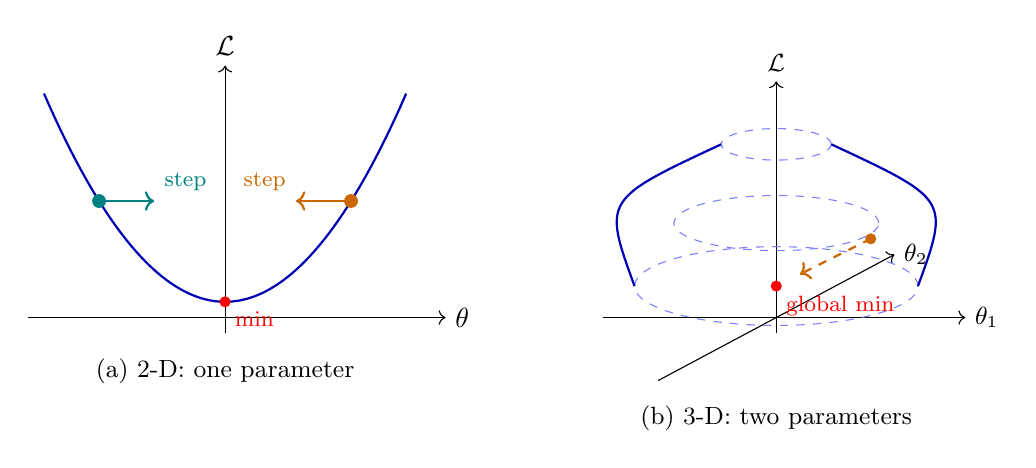
\begin{tikzpicture}
  %% ---- 2D loss curve (parabola-like) ----
  \begin{scope}[xshift=0cm]
    \draw[->] (-2.5,0) -- (2.8,0) node[right]{$\theta$};
    \draw[->] (0,-0.2) -- (0,3.2) node[above]{$\Loss$};
    %% parabola: y = (x)^2 * 0.5 + 0.2
    \draw[blue!70!black,thick,domain=-2.3:2.3,smooth,samples=60]
      plot (\x, {0.5*\x*\x + 0.2});
    %% minimum marker
    \fill[red] (0,0.2) circle (2pt) node[below right]{\footnotesize min};
    %% point on right slope
    \fill[orange!80!black] (1.6,{0.5*1.6*1.6+0.2}) circle (2.5pt);
    \draw[->,orange!80!black,thick]
      (1.6,{0.5*1.6*1.6+0.2}) -- +(-0.7,0)
      node[above left]{\footnotesize step};
    %% point on left slope
    \fill[teal] (-1.6,{0.5*1.6*1.6+0.2}) circle (2.5pt);
    \draw[->,teal,thick]
      (-1.6,{0.5*1.6*1.6+0.2}) -- +(0.7,0)
      node[above right]{\footnotesize step};
    \node[below] at (0,-0.4) {\small (a) 2-D: one parameter};
  \end{scope}

  %% ---- 3D bowl schematic ----
  \begin{scope}[xshift=7cm]
    %% axes
    \draw[->] (-2.2,0) -- (2.4,0) node[right]{\small$\theta_1$};
    \draw[->] (0,-0.2) -- (0,3.0) node[above]{\small$\Loss$};
    \draw[->] (-1.5,-0.8) -- (1.5,0.8) node[right]{\small$\theta_2$};
    %% ellipses to suggest a bowl
    \draw[blue!50,dashed] (0,0.4) ellipse (1.8cm and 0.5cm);
    \draw[blue!50,dashed] (0,1.2) ellipse (1.3cm and 0.35cm);
    \draw[blue!50,dashed] (0,2.2) ellipse (0.7cm and 0.2cm);
    %% bowl outline
    \draw[blue!70!black,thick]
      (-1.8,0.4) .. controls (-2.2,1.5) .. (-0.7,2.2);
    \draw[blue!70!black,thick]
      (1.8,0.4) .. controls (2.2,1.5) .. (0.7,2.2);
    %% minimum
    \fill[red] (0,0.4) circle (2pt) node[below right]{\footnotesize global min};
    %% gradient arrow
    \fill[orange!80!black] (1.2,1.0) circle (2pt);
    \draw[->,orange!80!black,thick,dashed] (1.2,1.0) -- (0.3,0.55);
    \node[below] at (0,-1.0) {\small (b) 3-D: two parameters};
  \end{scope}
\end{tikzpicture}
\caption{Loss landscape.
         (a) Convex 2-D curve: gradient descent steps (orange/teal arrows)
             always move toward the global minimum regardless of starting side.
         (b) Schematic 3-D bowl: the minimum occurs where all partial
             derivatives simultaneously equal zero.}
\label{fig:loss-landscape}
\end{figure}

\subsection{Multi-Dimensional Optimisation}

For a network with $n$ parameters the loss lives in an
$(n+1)$-dimensional space.
The minimum occurs when:
\begin{equation}
  \nabla_\Theta \Loss = \mathbf{0}
  \quad\Longleftrightarrow\quad
  \pderiv{\Loss}{\theta_i} = 0 \;\; \forall\, i = 1,\ldots,n.
  \label{eq:minimum-condition}
\end{equation}
Gradient descent iteratively approaches this point without requiring an
analytic solution of \cref{eq:minimum-condition}.

\begin{remark}
\label{rem:convex-vs-nonconvex}
For the squared-error loss used in this session, the loss landscape is
\emph{convex} with a unique global minimum (assuming fixed architecture and
data).
In practice, deep network loss landscapes are highly non-convex with many
local minima and saddle points.
However, empirical evidence shows that most local minima in deep networks
have similar loss values to the global minimum, and that gradient-based
methods find good solutions in practice.
\end{remark}

\subsection{The Role of Convergence}

\begin{definition}[Convergence]
\label{def:convergence}
Training is said to have \emph{converged} when parameter updates become
negligibly small:
\begin{equation}
  \|\theta^{(t+1)} - \theta^{(t)}\|
    = \eta\,\left\|\pderiv{\Loss}{\theta}\right\| < \varepsilon
  \label{eq:convergence}
\end{equation}
for a chosen tolerance $\varepsilon > 0$.
Equivalently, convergence can be declared when the loss ceases to decrease
significantly between iterations.
\end{definition}

% =============================================================================
\section{Learning Rate: Effects and Selection}
\label{sec:lr}
% =============================================================================

\subsection{Role of the Learning Rate}

The learning rate $\eta$ acts as a \emph{step-size multiplier}.
Together with the gradient, it determines how far the parameter moves in each
update.
Neither the gradient alone nor the learning rate alone is sufficient:
\begin{equation}
  \Delta\theta = -\eta\,\pderiv{\Loss}{\theta}.
  \label{eq:step}
\end{equation}

\subsection{Three Regimes}

\begin{table}[ht]
\centering
\caption{Effect of learning rate magnitude on training behaviour.}
\label{tab:lr-effects}
\begin{tabular}{p{2.5cm}p{4.5cm}p{5.5cm}}
\toprule
\textbf{Learning rate} & \textbf{Behaviour} & \textbf{Risk} \\
\midrule
Too small
  ($\eta \ll 1$) &
  Tiny steps; slow progress toward minimum. &
  Very slow convergence; may require millions of iterations. \\[6pt]
Moderate
  ($\eta \approx 0.01$) &
  Steady, stable descent toward minimum. &
  Best practical choice; may still require tuning. \\[6pt]
Too large
  ($\eta \gg 1$) &
  Overshoots the minimum; parameters jump to the opposite side. &
  Divergence or \emph{exploding gradients}; loss may increase. \\
\bottomrule
\end{tabular}
\end{table}

\begin{example}[Why $\eta = 10^{-4}$ was chosen in this session]
With gradients as large as 1413.12 (for $w_{11}$), a learning rate of
$\eta = 1$ would produce a parameter change of 1413 --- from $w_{11}=0.02$
to roughly $-1413$.
Using $\eta = 10^{-4}$ scales the largest step down to
$10^{-4} \times 1413 \approx 0.14$, a manageable change.
The instructor notes that the chosen learning rate is unusually small
precisely because the inputs $x_1=80$ and $x_2=8$ have very different scales.
The correct practice is to \emph{normalise inputs first}, then use a
moderate $\eta \approx 0.01$.
\end{example}

\begin{keyinsight}[title=Learning rate as speed control]
Think of the learning rate as a speed limit on the drive to the global
minimum.
If the speed is too low (small $\eta$), the journey takes too long.
If the speed is too high (large $\eta$), the driver overshoots the
destination and may end up on the opposite side.
A moderate speed allows reaching the destination reliably and in
reasonable time.
\end{keyinsight}

% =============================================================================
\section{Gradient Descent Variants}
\label{sec:gd-variants}
% =============================================================================

Once the gradient and update rule are understood for a single sample,
the question becomes: \emph{which data samples should drive each parameter
update?}
There are three standard answers.

\subsection{Batch Gradient Descent (BGD)}

Process \emph{all} $N$ training samples, accumulate the losses, then perform
one parameter update:
\begin{equation}
  \Loss_{\text{batch}} = \frac{1}{N}\sum_{i=1}^{N}\Loss(x^{(i)}, y^{(i)};\,\Theta),
  \label{eq:bgd-loss}
\end{equation}
\begin{equation}
  \theta \leftarrow \theta - \eta\,\pderiv{\Loss_{\text{batch}}}{\theta}.
  \label{eq:bgd-update}
\end{equation}

One pass through all $N$ samples plus one update is called one
\emph{epoch}.

\paragraph{Properties:}
\begin{itemize}[leftmargin=2em]
  \item Smooth, stable loss curve; gradient direction accurately reflects
        the entire dataset.
  \item Memory intensive: the entire dataset must fit in memory
        (or be streamed).
  \item Computationally expensive per update: $O(N)$ forward passes
        before any parameter change.
  \item Highly vectorisable; excellent GPU utilisation when $N$ is not
        too large.
\end{itemize}

\subsection{Stochastic Gradient Descent (SGD)}

Update parameters \emph{after every single sample}:
\begin{equation}
  \theta \leftarrow \theta - \eta\,\pderiv{\Loss(x^{(i)}, y^{(i)};\,\Theta)}{\theta}
  \quad \text{for each } i = 1, \ldots, N.
  \label{eq:sgd-update}
\end{equation}
In one epoch there are $N$ parameter updates.

\paragraph{Properties:}
\begin{itemize}[leftmargin=2em]
  \item Very fast per-update; parameters change after every single sample.
  \item High variance: the loss curve is noisy and zigzag because each
        sample provides only a partial view of the true gradient.
  \item Can escape shallow local minima due to noisy updates.
  \item Poor vectorisation: only one sample processed at a time.
  \item Convergence in terms of \emph{number of parameter updates} is fast,
        but wall-clock time may exceed BGD because of 1000$\times$ more
        gradient computations per epoch.
\end{itemize}

\subsection{Mini-Batch Gradient Descent (MBGD)}

Process $M$ samples (the \emph{mini-batch}) at a time:
\begin{equation}
  \Loss_{\text{mini}} = \frac{1}{M}\sum_{i \in \mathcal{B}}\Loss(x^{(i)}, y^{(i)};\,\Theta),
  \label{eq:mbgd-loss}
\end{equation}
\begin{equation}
  \theta \leftarrow \theta - \eta\,\pderiv{\Loss_{\text{mini}}}{\theta}.
  \label{eq:mbgd-update}
\end{equation}
With $N=100$ samples and $M=10$, there are 10 updates per epoch.

\paragraph{Properties:}
\begin{itemize}[leftmargin=2em]
  \item \textbf{Best of both worlds}: more stable than SGD, faster than BGD.
  \item GPU-friendly: batch size $M$ is chosen to fit in GPU memory.
  \item Typical values: $M \in \{16, 32, 64, 128, 256\}$.
  \item The \emph{de facto} standard in modern deep learning.
\end{itemize}

\subsection{Comparison Table}

\begin{table}[ht]
\centering
\caption{Comparison of gradient descent variants.
         $N$ = dataset size; $M$ = mini-batch size; $T$ = epochs.}
\label{tab:gd-comparison}
\begin{tabularx}{\linewidth}{lXXXX}
\toprule
\textbf{Variant} &
\textbf{Samples per update} &
\textbf{Updates per epoch} &
\textbf{Convergence} &
\textbf{Vectorisation} \\
\midrule
BGD  & $N$ (all) & 1         & Smooth, slow  & Excellent \\
SGD  & 1         & $N$       & Noisy, fast   & Poor      \\
MBGD & $M$       & $N/M$     & Balanced      & Good (GPU)\\
\bottomrule
\end{tabularx}
\end{table}

\subsection{Convergence Trajectories}

\begin{figure}[ht]
\centering
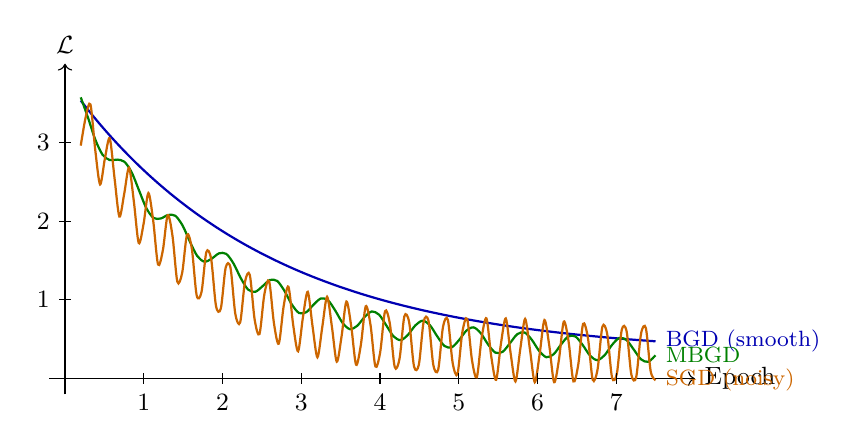
\begin{tikzpicture}[font=\small]
  \draw[->] (-0.2,0) -- (8,0) node[right]{Epoch};
  \draw[->] (0,-0.2) -- (0,4) node[above]{$\Loss$};

  %% BGD: smooth curve
  \draw[blue!70!black,thick,domain=0.2:7.5,smooth,samples=60]
    plot (\x, {3.5*exp(-0.4*\x)+0.3})
    node[right]{\footnotesize BGD (smooth)};

  %% MBGD: slightly noisy
  \draw[green!50!black,thick,domain=0.2:7.5,smooth,samples=80]
    plot (\x, {3.5*exp(-0.55*\x) + 0.3 + 0.15*sin(10*\x r)})
    node[right]{\footnotesize MBGD};

  %% SGD: very noisy
  \draw[orange!80!black,thick,domain=0.2:7.5,smooth,samples=120]
    plot (\x, {3.5*exp(-0.7*\x) + 0.3 + 0.4*sin(25*\x r)})
    node[right]{\footnotesize SGD (noisy)};

  %% axis ticks
  \foreach \x in {1,2,3,4,5,6,7}
    \draw (\x,2pt) -- (\x,-2pt) node[below]{\x};
  \foreach \y in {1,2,3}
    \draw (2pt,\y) -- (-2pt,\y) node[left]{\y};
\end{tikzpicture}
\caption{Schematic loss curves for the three gradient descent variants.
         BGD is smooth but slow to converge per epoch.
         SGD converges fastest in terms of parameter updates but is noisy.
         MBGD provides a practical balance.}
\label{fig:loss-curves}
\end{figure}

\begin{remark}
\label{rem:sgd-escape}
The noise in SGD is not always harmful: the random fluctuations can help
the optimiser escape shallow local minima.
This \emph{implicit regularisation} effect of SGD/MBGD is one reason why
small batch sizes are still used in practice even when larger batches would
fit in memory.
\end{remark}

% =============================================================================
\section{PyTorch Implementation Notes}
\label{sec:pytorch}
% =============================================================================

The session includes a live coding demonstration.
The key PyTorch patterns are outlined below.

\subsection{Data Generation}

The instructor creates a synthetic 500-sample IQ/CGPA$\to$LPA dataset:

\begin{verbatim}
import torch
N = 500
torch.manual_seed(42)
IQ   = torch.randint(50, 130, (N, 1)).float()
CGPA = 5 + 5 * torch.rand(N, 1)
X = torch.cat([IQ, CGPA], dim=1)   # shape: (500, 2)
Y = 0.1*IQ + 0.5*CGPA + 0.01*torch.randn(N,1)
\end{verbatim}

\subsection{Manual Parameter Initialisation}

Nine parameters are created with \texttt{requires\_grad=True} so that
PyTorch's autograd engine can compute their gradients automatically:

\begin{verbatim}
params = [
    torch.tensor([[0.02]], requires_grad=True),  # w11
    torch.tensor([[0.50]], requires_grad=True),  # w12
    ...  # (all 9 parameters)
]
\end{verbatim}

\subsection{Training Loop Skeleton}

\begin{verbatim}
lr = 1e-4
for epoch in range(200):
    # Forward pass
    z1 = X[:,0:1]*params[0] + X[:,1:2]*params[1] + params[4]
    h1 = torch.relu(z1)
    z2 = X[:,0:1]*params[2] + X[:,1:2]*params[3] + params[5]
    h2 = torch.relu(z2)
    yhat = params[6]*h1 + params[7]*h2 + params[8]
    loss = ((yhat - Y)**2).mean()

    # Backward pass
    loss.backward()

    # Parameter update (manual)
    with torch.no_grad():
        for p in params:
            p -= lr * p.grad
            p.grad.zero_()
\end{verbatim}

\begin{keyinsight}[title=Gradient zeroing]
The call \texttt{p.grad.zero\_()} after each update is mandatory.
PyTorch accumulates (adds) gradients by default.
Without zeroing, gradient from iteration $t-1$ would be added to the
gradient at iteration $t$, corrupting the update.
\end{keyinsight}

\subsection{Switching Between Gradient Descent Variants}

\begin{table}[ht]
\centering
\caption{How to implement each GD variant in PyTorch by adjusting the
         \texttt{DataLoader} batch size.}
\label{tab:pytorch-gd}
\begin{tabular}{lll}
\toprule
\textbf{Variant} & \textbf{DataLoader setting} & \textbf{Updates per epoch} \\
\midrule
BGD  & \texttt{batch\_size=N} (full dataset) & 1 \\
SGD  & \texttt{batch\_size=1}                & $N$ \\
MBGD & \texttt{batch\_size=32} (or 64, 128)  & $\lceil N/32 \rceil$ \\
\bottomrule
\end{tabular}
\end{table}

% =============================================================================
\section{Summary and Conclusions}
\label{sec:summary}
% =============================================================================

\subsection{Session Recap}

Session~07 provided a fully numerical end-to-end demonstration of the
backpropagation algorithm on the canonical 2-2-1 network, and established the
conceptual framework needed for training deeper networks.
The key steps were:

\begin{enumerate}[leftmargin=2em,label=\textbf{\arabic*.}]
  \item \textbf{Forward pass} ($x_1=80$, $x_2=8$, $y=3$): produced
        $\yhat = 10.36$, $\Loss = 54.17$.
  \item \textbf{Backward pass}: computed all 9 gradients using the chain
        rule.  The largest gradient ($\pderiv{\Loss}{w_{11}} = 1413.12$) arose
        because $x_1 = 80$ amplifies every factor in the chain-rule product.
  \item \textbf{Parameter update} ($\eta = 10^{-4}$): all 9 parameters
        updated simultaneously; new loss $= 4.006$ --- a 92.6\% reduction in
        one step.
  \item \textbf{Gradient concept}: gradient is slope; gradient descent
        subtracts a scaled slope, always moving downhill regardless of which
        side of the minimum the current point is on.
  \item \textbf{Gradient descent variants}: BGD (stable, slow), SGD (noisy,
        fast), MBGD (balanced, GPU-friendly).
\end{enumerate}

\subsection{Key Takeaways}

\begin{table}[ht]
\centering
\caption{Core messages from Session~07 and their implications for practice.}
\label{tab:takeaways}
\begin{tabularx}{\linewidth}{p{4cm}X}
\toprule
\textbf{Concept} & \textbf{Practical implication} \\
\midrule
Chain rule drives backprop &
  Every parameter is reachable via the chain rule; no special treatment
  needed for deeply buried weights. \\[4pt]
Input scale $\to$ gradient scale &
  Normalise features before training to prevent pathologically large
  gradients for weights connected to large-valued inputs. \\[4pt]
Learning rate controls step size &
  Tune $\eta$; neither too large (diverge) nor too small (slow).
  Common starting points: $0.01$--$0.001$. \\[4pt]
Dead ReLU after large steps &
  Overshooting can kill ReLU neurons.
  Use proper weight initialisation and gradient clipping. \\[4pt]
MBGD is the default &
  Mini-batch gradient descent with batch size 32--256 balances
  speed, stability, and GPU memory. \\
\bottomrule
\end{tabularx}
\end{table}

\subsection{Looking Ahead}

The next sessions will build on these foundations to cover:
\begin{itemize}[leftmargin=2em]
  \item The \textbf{vanishing gradient problem} and how it arises when
        deep networks use sigmoid or tanh activations.
  \item Solutions: ReLU family, batch normalisation, residual connections.
  \item The \texttt{torch.nn} module for building networks without manual
        parameter management.
  \item The \texttt{torch.optim} module, which encapsulates the update rule
        and supports advanced optimisers (Adam, RMSProp, Momentum SGD).
  \item Convolutional Neural Networks (CNN), Recurrent Neural Networks
        (RNN), and Long Short-Term Memory (LSTM) networks, where the same
        chain-rule mechanics apply.
\end{itemize}

\begin{keyinsight}[title=Universality of backpropagation]
Every concept introduced in this session --- chain rule, gradient
computation, learning rate, mini-batch processing --- applies unchanged to
CNN, RNN, and Transformer architectures.
The only difference is the \emph{form} of the forward-pass equations;
the backward pass machinery is always the same.
\end{keyinsight}

\end{document}
